\documentclass[10pt]{homeworg}

\usepackage{bm}
\title{Homework 3}
\author{Kevin Yang - 50244152}


\begin{document}

\maketitle

\Huge{Link to repo:}\\
\Large{https://github.com/keviny2/CPSC532W-Assignments/tree/main/FOPPL}

\section{Program 0}
BBVI implementation:
\begin{center}
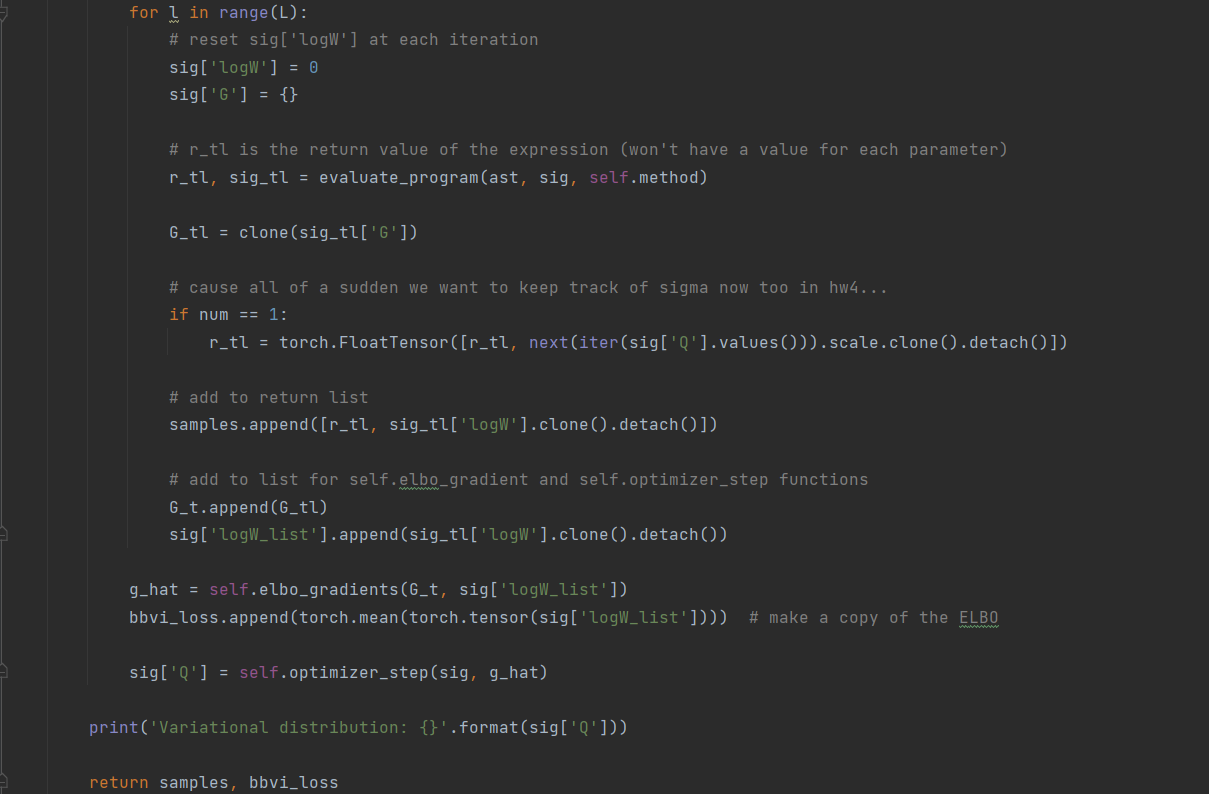
\includegraphics[scale=0.5]{figures/bbvi.png}
\end{center}

\newpage

\begin{center}
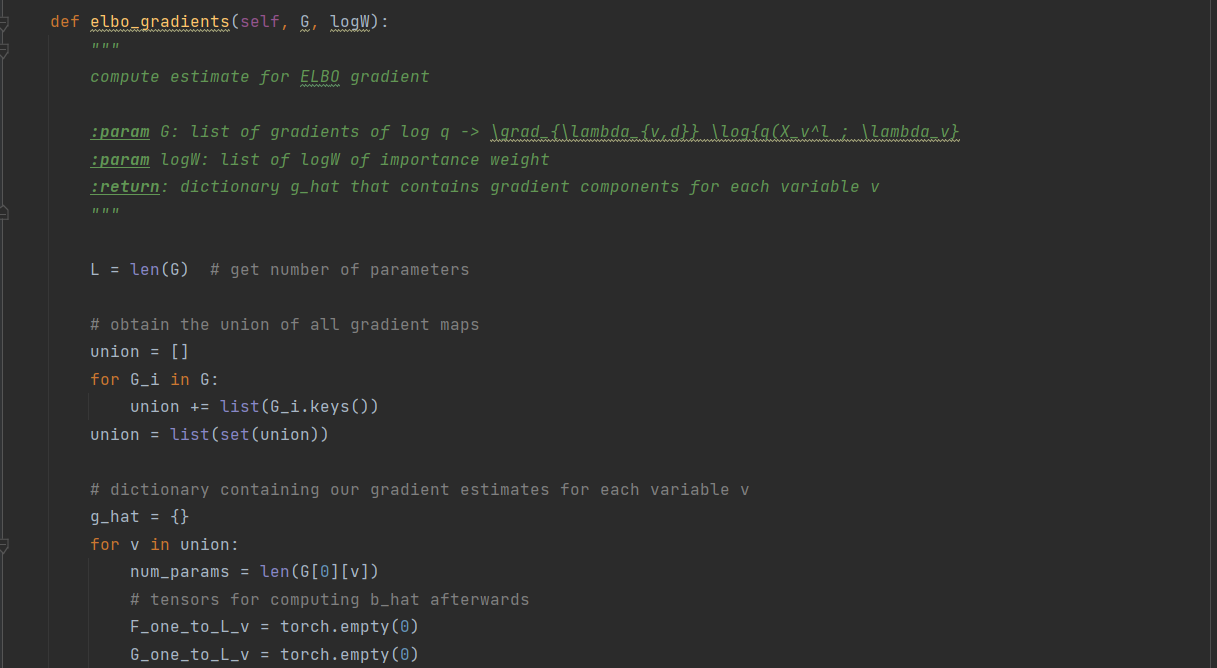
\includegraphics[scale=0.5]{figures/elbo_gradients_1.png}
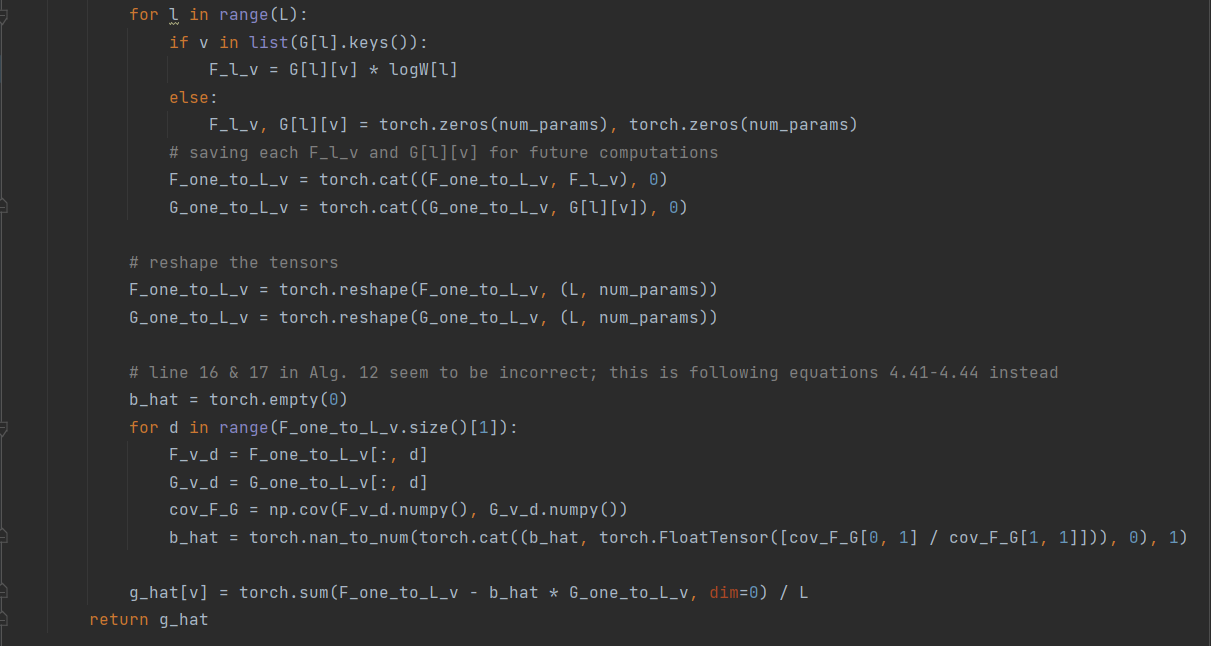
\includegraphics[scale=0.5]{figures/elbo_gradients_2.png}
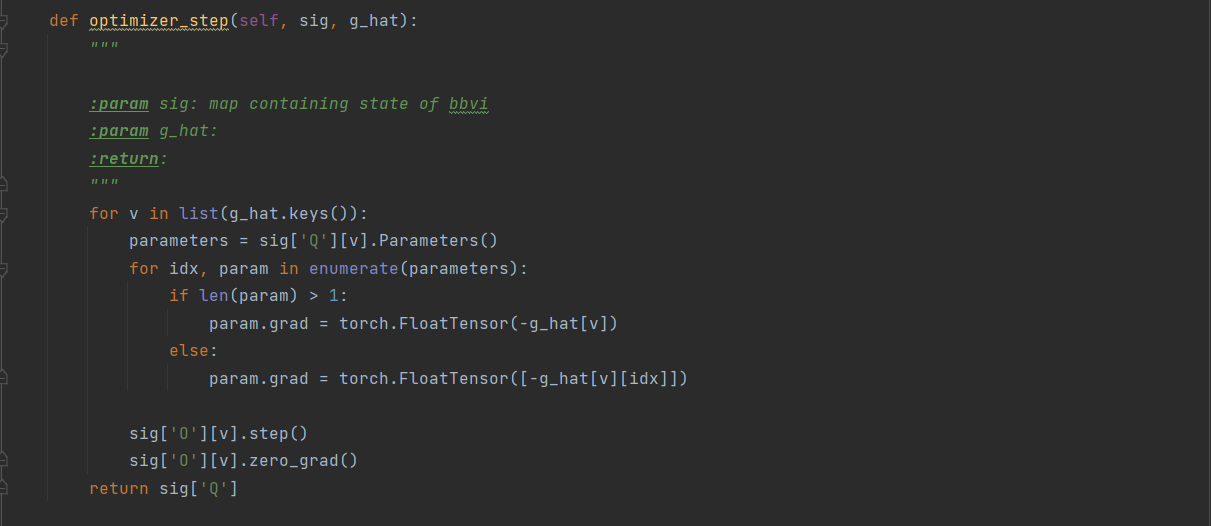
\includegraphics[scale=0.5]{figures/optimizer_step.png}
\end{center}


\section{Program 1}
\begin{center}
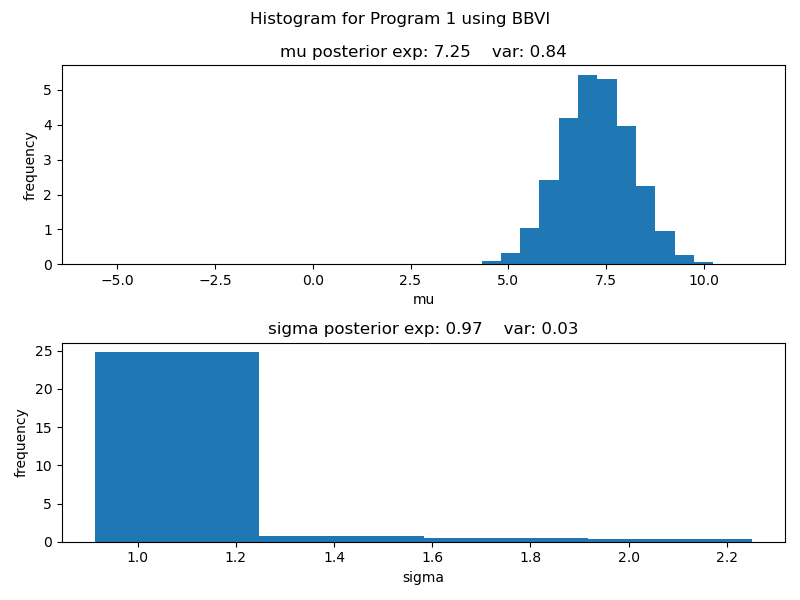
\includegraphics[scale=0.5]{figures/BBVI_program_1.png}
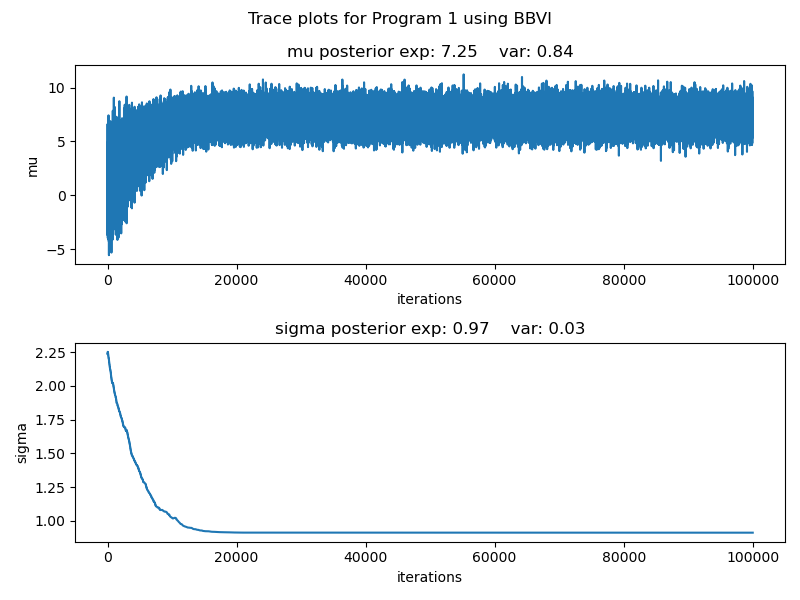
\includegraphics[scale=0.5]{figures/BBVI_program_1_trace.png}
\end{center}

\begin{figure}[!htbp]
    \centering
    \begin{minipage}{0.45\textwidth}
        \centering
       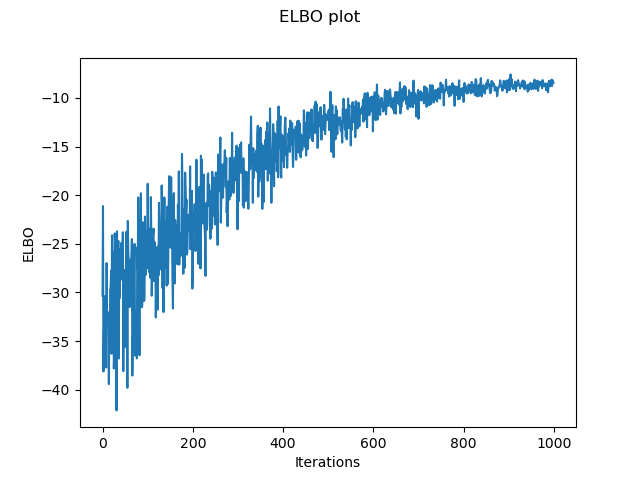
\includegraphics[scale=0.5]{figures/elbo_program_1.png}
    \end{minipage}\hfill
    \begin{minipage}{0.45\textwidth}
        \centering
        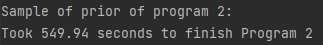
\includegraphics[scale=0.8]{figures/program1_time.png}
    \end{minipage}
\end{figure}

\newpage

%%%%%%%%%%%%%%%%%%%%%%%%%%%%%%%%%%%%%%%%%%%%%%%%%%%%%%

\section{Program 2}
\begin{center}
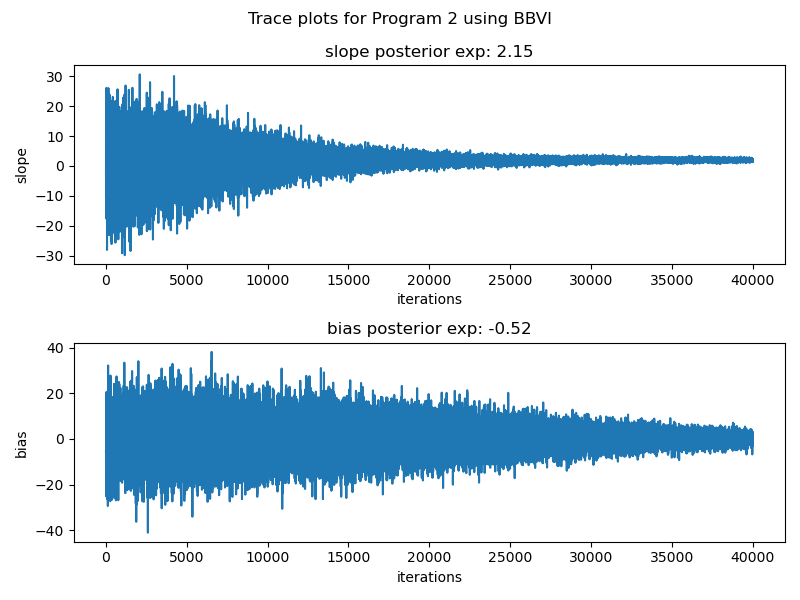
\includegraphics[scale=0.5]{figures/BBVI_program_2.png}
\end{center}

\begin{figure}[!htbp]
    \centering
    \begin{minipage}{0.45\textwidth}
        \centering
       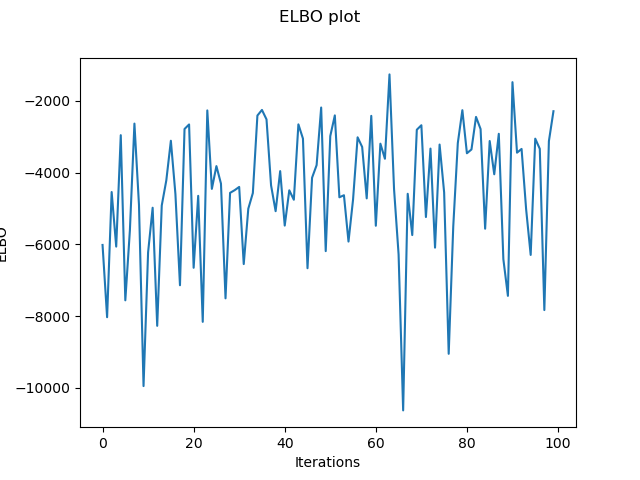
\includegraphics[scale=0.5]{figures/elbo_program_2.png}
    \end{minipage}\hfill
    \begin{minipage}{0.45\textwidth}
        \centering
        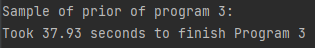
\includegraphics[scale=0.8]{figures/program2_time.png}
    \end{minipage}
\end{figure}


%%%%%%%%%%%%%%%%%%%%%%%%%%%%%%%%%%%%%%%%%%%%%%%%%%%%%%

\section{Program 3}
\begin{center}
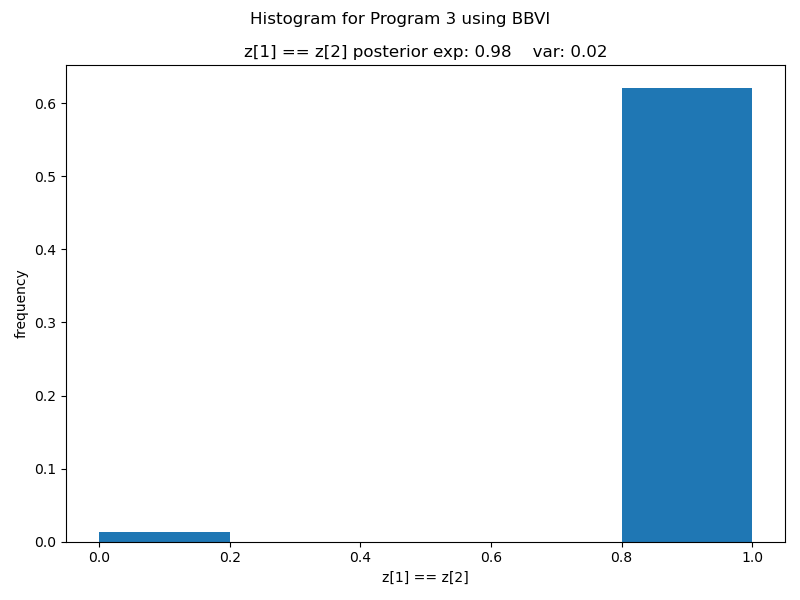
\includegraphics[scale=0.5]{figures/BBVI_program_3.png}
\end{center}

\begin{figure}[!htbp]
    \centering
    \begin{minipage}{0.45\textwidth}
        \centering
       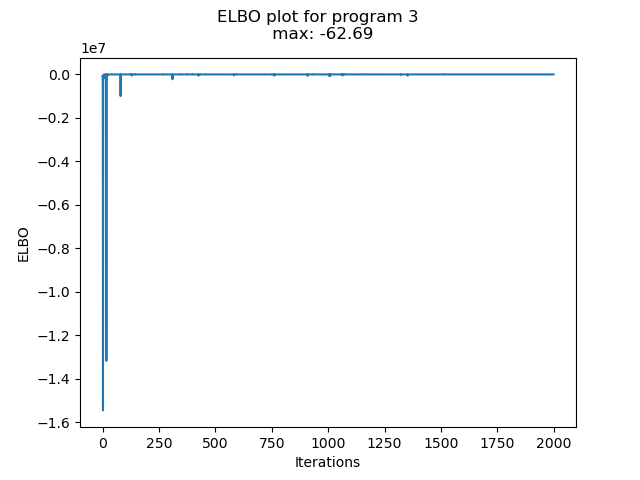
\includegraphics[scale=0.5]{figures/elbo_program_3.png}
    \end{minipage}\hfill
    \begin{minipage}{0.45\textwidth}
        \centering
        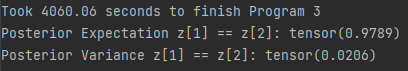
\includegraphics[scale=0.8]{figures/program3_time.png}
    \end{minipage}
\end{figure}

The mode-seeking behavior of VI on models with internal symmetries will find itself climbing different modes in the posterior for independent runs. These internal symmetries render the model unidentifiable, because the model density is invariant under some classes of transformations of the latent parameter (Moore, 2016). This reduces the efficiency of inference procedures. The label switching problem is a well known problem in mixture models, as the latent variables representing class labels are unidentifiable in the sense that the model density does not change if you swap the labels of two classes - hence, \textit{unidentifiable}.


%%%%%%%%%%%%%%%%%%%%%%%%%%%%%%%%%%%%%%%%%%%%%%%%%%%%%%

\section{Program 4}
\begin{figure}[!htbp]
    \centering
    \begin{minipage}{0.45\textwidth}
        \centering
       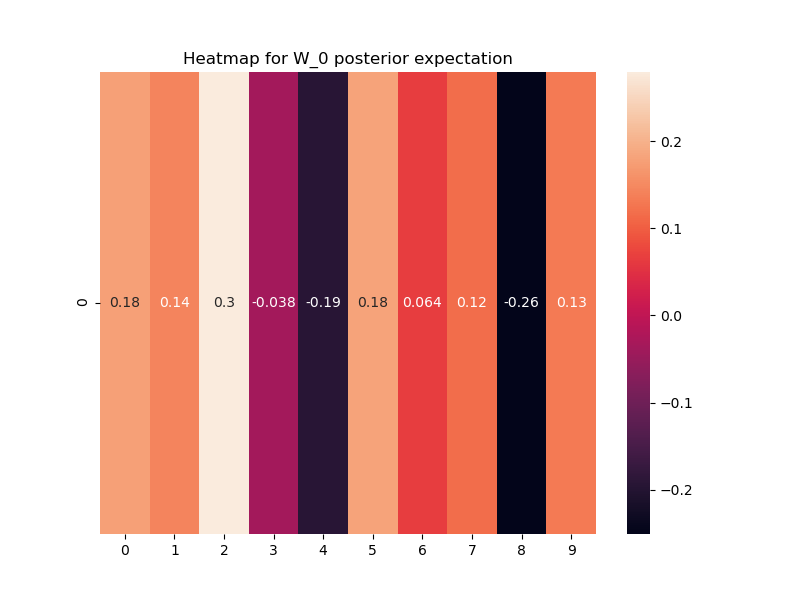
\includegraphics[scale=0.5]{figures/heatmap_exp_W_0.png}
    \end{minipage}\hfill
    \begin{minipage}{0.45\textwidth}
        \centering
        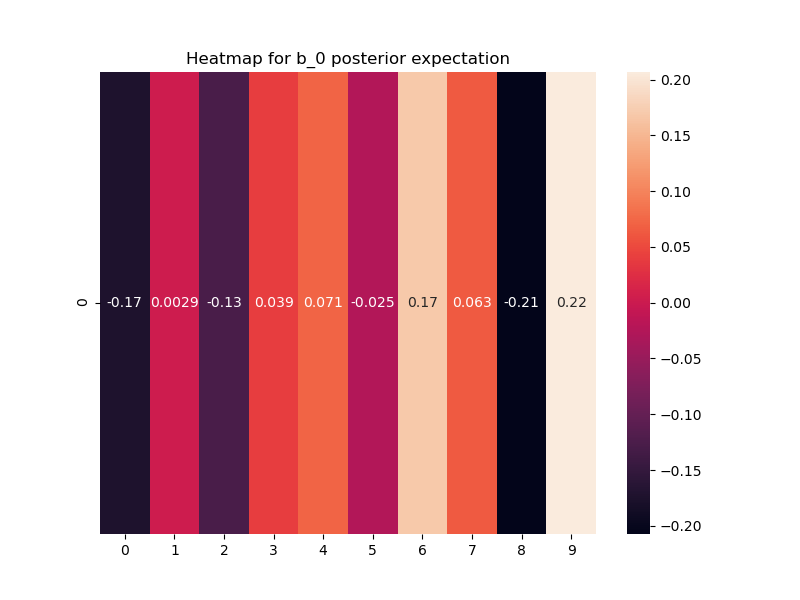
\includegraphics[scale=0.5]{figures/heatmap_exp_b_0.png}
    \end{minipage}
\end{figure}

\begin{figure}[!htbp]
    \centering
    \begin{minipage}{0.45\textwidth}
        \centering
       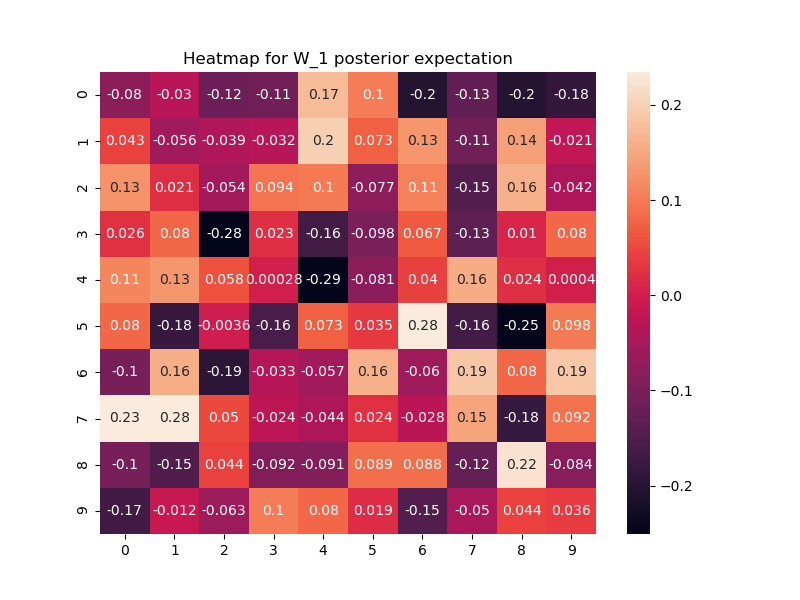
\includegraphics[scale=0.5]{figures/heatmap_exp_W_1.png}
    \end{minipage}\hfill
    \begin{minipage}{0.45\textwidth}
        \centering
        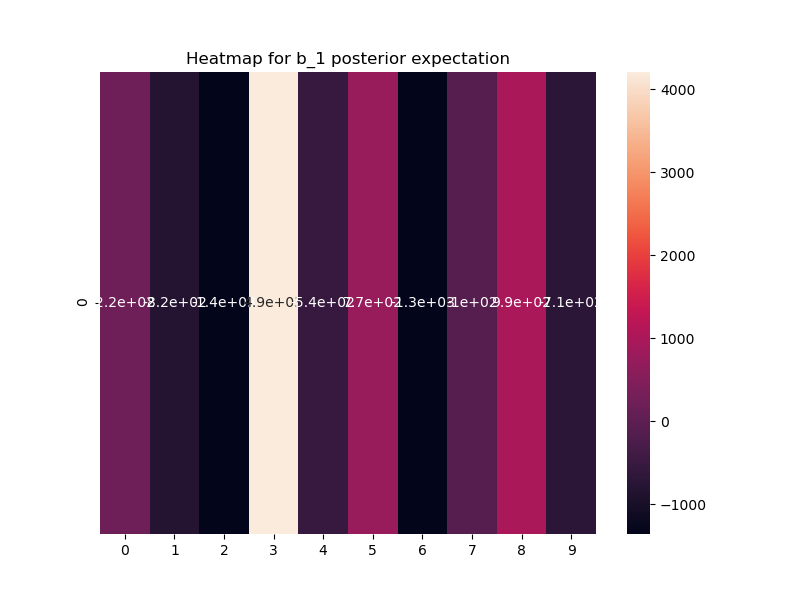
\includegraphics[scale=0.5]{figures/heatmap_exp_b_1.png}
    \end{minipage}
\end{figure}

\newpage

\begin{figure}[!htbp]
    \centering
    \begin{minipage}{0.45\textwidth}
        \centering
       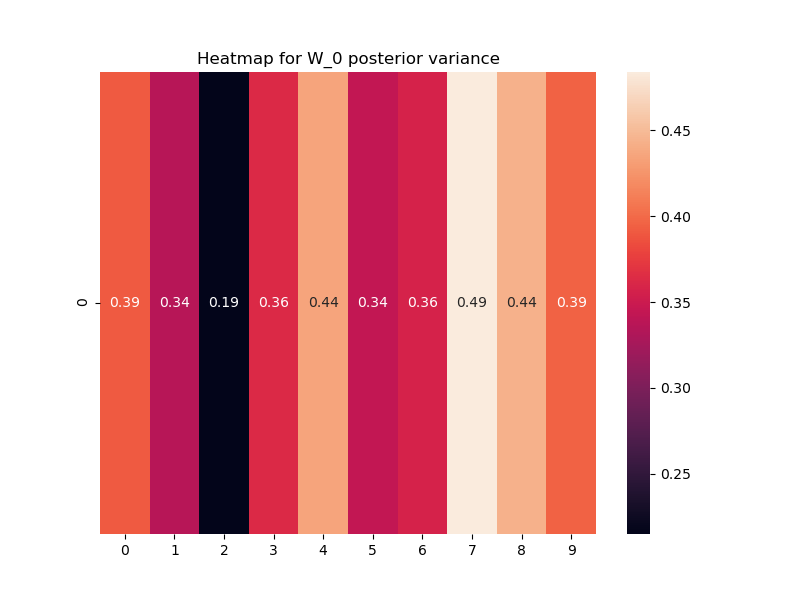
\includegraphics[scale=0.5]{figures/heatmap_var_W_0.png}
    \end{minipage}\hfill
    \begin{minipage}{0.45\textwidth}
        \centering
        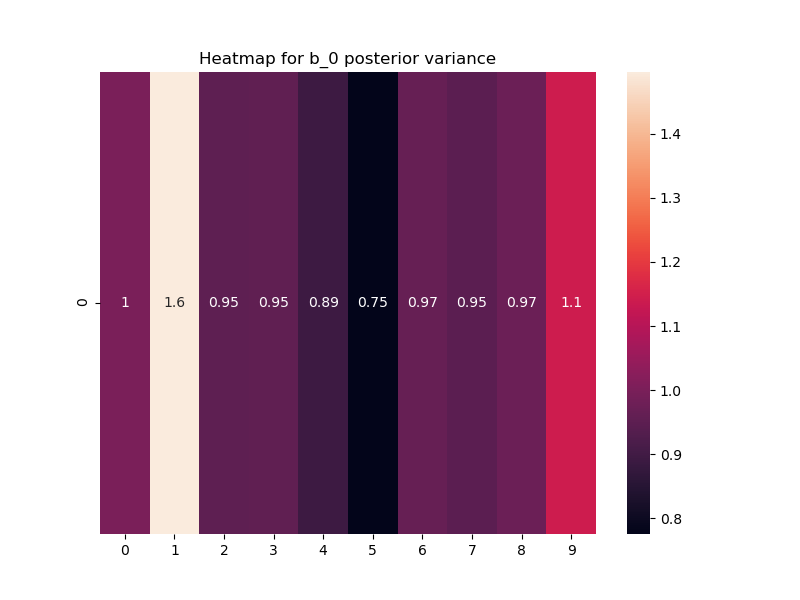
\includegraphics[scale=0.5]{figures/heatmap_var_b_0.png}
    \end{minipage}
\end{figure}

\begin{figure}[!htbp]
    \centering
    \begin{minipage}{0.45\textwidth}
        \centering
       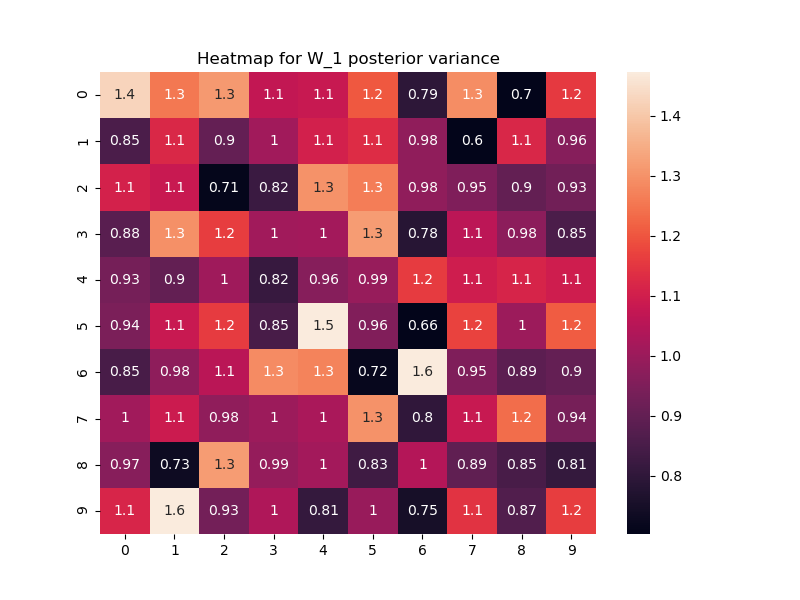
\includegraphics[scale=0.5]{figures/heatmap_var_W_1.png}
    \end{minipage}\hfill
    \begin{minipage}{0.45\textwidth}
        \centering
        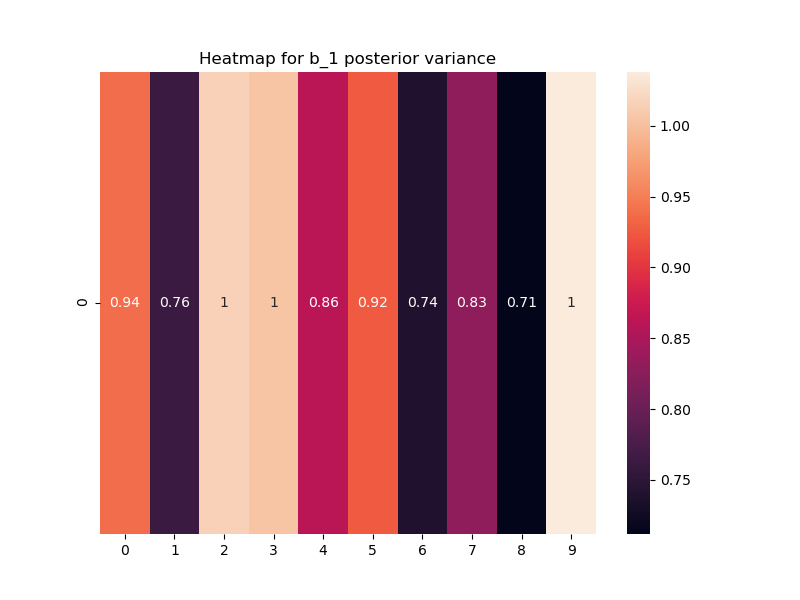
\includegraphics[scale=0.5]{figures/heatmap_var_b_1.png}
    \end{minipage}
\end{figure}

\begin{figure}[!htbp]
    \centering
    \begin{minipage}{0.45\textwidth}
        \centering
       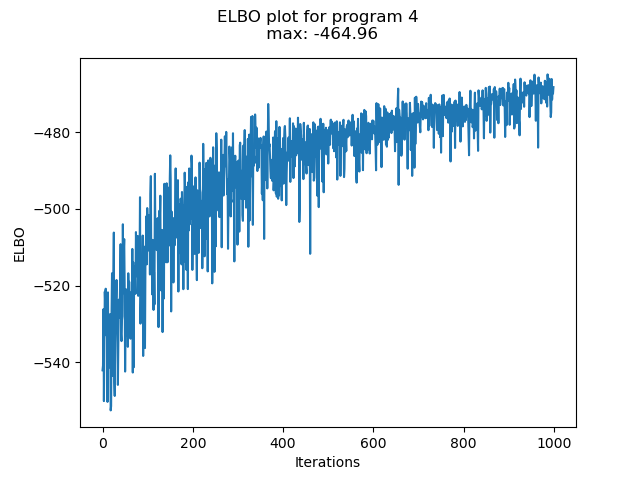
\includegraphics[scale=0.5]{figures/elbo_program_4.png}
    \end{minipage}\hfill
    \begin{minipage}{0.45\textwidth}
        \centering
        
\includegraphics[scale=0.8]{figures/program4_time.png}
    \end{minipage}
\end{figure}

\newpage

Black-box variational inference (BBVI) is more generic compared to parameter estimation via gradient descent. In BBVI, we compute an estimate of the gradient of the evidence lower bound (ELBO) using a sampling procedure instead of obtaining the gradient of the ELBO analytically. This renders BBVI applicable to a range of complicated models that parameter estimation via gradient descent will not be able to handle.

%%%%%%%%%%%%%%%%%%%%%%%%%%%%%%%%%%%%%%%%%%%%%%%%%%%%%%

\section{Program 5}

The variational distribution is a Gamma(7.79, 1.32)

\begin{figure}[!htbp]
    \centering
    \begin{minipage}{0.5\textwidth}
        \centering
       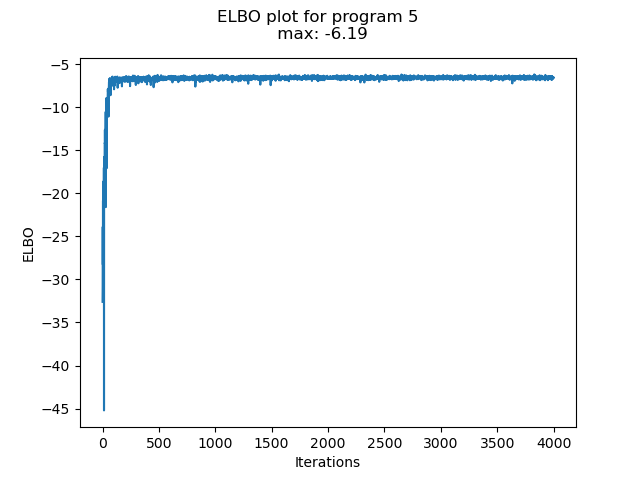
\includegraphics[scale=0.5]{figures/elbo_program_5.png}
    \end{minipage}\hfill
    \begin{minipage}{0.5\textwidth}
        \centering
        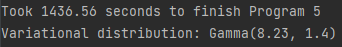
\includegraphics[scale=0.8]{figures/program5_time.png}
    \end{minipage}
\end{figure}

\section{References}
Moore, D. A. (2016) \textit{Symmetrized Variational Inference}. NIPS Workshop on Advances in Approximate Inference.

\end{document}